\documentclass[a4paper,twocolumn,10pt]{article}
\usepackage[spanish]{babel}
\usepackage[latin1]{inputenc}
\usepackage{graphicx}
\usepackage{flushend}
\usepackage{enumerate}

\begin{document}

\title{Guia de Seguridad de Base de Datos}
\author{\begin{tabular}{c c c c c c }
Brandon M. &  Angelo Q. & Jhordy V. & Leidy H. & Angela B. & Mreya P. \\
(2015052715) & (2015052826) & (2015052719) & (2015053230) & (2016054494) & (2015053234)\\
\end{tabular}
\\}

\date{}

\twocolumn[
\begin{@twocolumnfalse}
\maketitle
\vspace*{-1cm}
\begin{center}\rule{1\textwidth}{0.1mm} \end{center}



\begin{abstract}
\normalsize La seguridad de la base de datos se refiere al uso de una amplia gama de controles de seguridad de la informaci\'on para proteger las bases de datos (que pueden incluir los datos, las aplicaciones de la base de datos o las funciones almacenadas, los sistemas de la base de datos, los servidores de la base de datos y los enlaces de red asociados) contra el compromiso de su confidencialidad, integridad y disponibilidad. Implica varios tipos o categor\'ias de controles, tales como t\'ecnicos, de procedimiento / administrativos y f\'isicos. La seguridad de la base de datos es un tema especializado dentro de los \'ambitos m\'as amplios de la seguridad inform\'atica , la seguridad de la informaci\'on y la gesti\'on de riesgos. 
\begin{center}\rule{0.9\textwidth}{0.1mm} \end{center}
\vspace*{0.5cm}
\end{abstract}
\end{@twocolumnfalse}
]

\section{Introducci\'on}
\normalsize En el presente informe Se explicara c\'omo es que se debe realizar un respaldo de la informaci\'on, en este caso el respaldo de una base de datos en Oracle 11g Enterprise Edition para el uso del asistente grafico para copias de seguridad (Enterprise Manager).
\normalsize Adem\'as se utilizara SQLDEVElOPER.exe para para conectar un usuario, tambi\'en sirve para migraci\'on de bases de datos de MySQL a Oracle.
\normalsize Se explicara qu\'e tipos de backups se pueden realizar en Oracle, algunas recomendaciones de cuando realizar las copias de seguridad adem\'as de copias de seguridad en modo consola y de manera gr\'afica.


\section{Objetivos}

    \subsection{Generales}
       \normalsize Desarrollar una Gui\'ia T\'ecnica de estrategia de copias de Seguridad y Recuperaci\'on de Bases de Datos.
    \subsection{Especificos}
       \normalsize Definir que tipo de Backup aplicar y en que consiste cada uno . Explicar el impacto de las estrategias de Backups en las necesidades del espacio.

\section{Marco Te\'orico}
	 \subsection{Copias de seguridad y restauracion de base de datos}
\normalsize Una copia de los datos que se puede utilizar para restaurar y recuperar los datos se denomina copia de seguridad. Las copias de seguridad le permiten restaurar los datos despu\'es de un error. Con las copias de seguridad correctas puede recuperarse de multitud de errores por ejemplo
		\normalsize Errores de medios
		\normalsize Errores de usuario
		\normalsize Desastres naturales

	 \subsection{COMO IMPEDIR LA PERDIDA DE DATOS}
\normalsize Impedir la p\'erdida de datos es uno de los problemas m\'as importantes que afrontan los administradores de sistemas.\\

   \begin{enumerate}[a)]
        \item Disponer de una estrategia de copia de seguridad

\normalsize Debe tener una estrategia de copia de seguridad para aminorar la p\'erdida de datos y recuperar los datos perdidos. Los datos se pueden perder como consecuencia de errores de hardware o de software, o bien por:\\

\normalsize Virus destructivos.
\normalsize Desastres naturales, como incendios, inundaciones y terremotos.
\normalsize Robo.\\

      \item  Hacer copias de seguridad con regularidad
La frecuencia con que haga las copias de seguridad de la base de datos depende de la cantidad de datos que est\'e dispuesto a perder y la actividad de la base de datos. Cuando haga copias de seguridad de bases de datos de usuario, tenga en cuenta los siguientes hechos e instrucciones:
 \renewcommand{\labelitemi}{$-$}
\renewcommand{\labelitemii}{$\cdot$}
    \begin{itemize}
    \item Puede hacer copias de seguridad de la base de datos con frecuencia si el sistema se encuentra en un entorno de proceso de transacciones en l\'inea (OLTP, Online Transaction Processing).
    \item Puede hacer copias de seguridad de la base de datos con menos frecuencia si el sistema tiene poca actividad o se utiliza, principalmente, para la toma de decisiones.
    \item Debe programar las copias de seguridad cuando no se est\'en efectuando muchas actualizaciones en SQL Server.
    
   \end{itemize}

 \end{enumerate}
\renewcommand{\labelitemi}{$-$}
\renewcommand{\labelitemii}{$\cdot$}

\begin{enumerate}[a)]
    \item Tipos de Respaldo que Soporta Oracle
   \begin{itemize}
          \item Completo.- Se respalda toda la base de datos.
          \item Incremental.- Debe tener previamente un respaldo completo. Respalda a medida que se realizan cambios.
          \item 	Diferencial.- Debe tener previamente un respaldo completo. Respalda las diferencias existentes entre un respaldo y otro.
          \item Flashbacks.- Permite de manera rápida volver a un estado anterior de la base de datos.
          \item Respaldo y Recuperacion
          \item Para determinar cu\'ando hacer un respaldo, pensar de la siguiente manera: hacer una copia de respaldo justo antes del momento en que regenerar los datos ocasione mayor esfuerzo que hacer el respaldo.
       \end{itemize}
   \item Respaldos
      \normalsize Respaldo es la obtencion de una copia de los datos en otro medio magnetico, de tal modo que a partir de dicha copia es posible restaurar el sistema al momento de haber realizado el respaldo. Por lo tanto, los respaldos deben hacerse con regularidad, con la frecuencia preestablecida y de la manera indicada, a efectos de hacerlos correctamente. Es fundamental hacer bien los respaldos . De nada sirven respaldos mal hechos (por ejemplo, incompletos). En realidad , es peor disponer de respaldos no confiables que carecer totalmente de ellos. \\
 Suele ocurrir que la realizaci\'on de respaldos es una tarea relegada a un plano secundario, cuando en realidad la continuidad de una aplicacion depende de los mismos. Los respaldos son tan importantes como lo es el correcto ingreso de datos.
\end{enumerate}

\section{Desarrollo}
\begin{enumerate}[4.1]
\item  PROCEDIMIENTOS PARA LA CREACI\'ON DE COPIAS:
\\Primero se instal\'o la base de datos Oracle
\\Oracle Database 11g Release 2\\
\\Standard Edition, Standard Edition One, and Enterprise Edition para Windows\\
\\
- http://www.oracle.com/technetwork/database/enterprise-edition/downloads/112010-win64soft-094461.html\\
\\
\\Segundo se utiliz\'o el programa sql developer para windows, esto fue para migrar la base de datos de mysql a oracle.
\\Si es que se requiera cambiar el puerto  oracle exec DBMS
\\
\\- https://www.youtube.com/watch?v=-LJ\_370\_88g
\\Las copias de seguridad o backups pueden ser fisicas y logicas
\\
\\-Las fisicas se realizan cuando se copian los ficheros que soportan la BD
\\ Entre estos se encuentran los backups del SO, los backups en frio y los backups en caliente.
\\
\textbf{ Backups del SO}         
\\           Este tipo de backup implica parar la BD en modo normal y esto la hace inaccesible el sistema mientras se lleva a cabo.
\\
\\
\textbf{ Backups de la BD en Frio}         
\\          Los backups en frio implican parar la BD en modo normal y copiar todos los ficheros sobre los que se asienta. Antes de parar la BD hay que parar tambien todas las aplicaciones que esten trabajando con la BD. Una vez realizada la copia de los ficheros, la BD se puede volver a arrancar.
\\
\\
\textbf{Backups de la BD en Caliente}            
\\          El backup en caliente se realiza mientras la BD esta abierta y funcionando en modo ARCHIVELOG. Habra que tener cuidado de realizarlo cuando la carga de la BD sea chica. Este tipo de backup consiste en copiar todos los ficheros correspondientes a un tablespace determinado, los ficheros redo log archivados y los ficheros de control.
\\

	\textbf{Backups Logicos con Export, Import}  
	\\Estas utilidades permiten al DBA hacer copias de determinados objetos de la BD, asi como restaurarlos o moverlos de una BD a otra. Estas herramientas utilizan comandos del SQL para obtener el contenido de los objetos.\\
	\\
	\\NOTA: Una vez que se ha planeado una estrategia de backup y se ha probado, conviene automatizarla para facilitar asi su cumplimiento.



\item BACKUPS  DESDE  ENTERPRISE  MANAGER

\begin{center}
	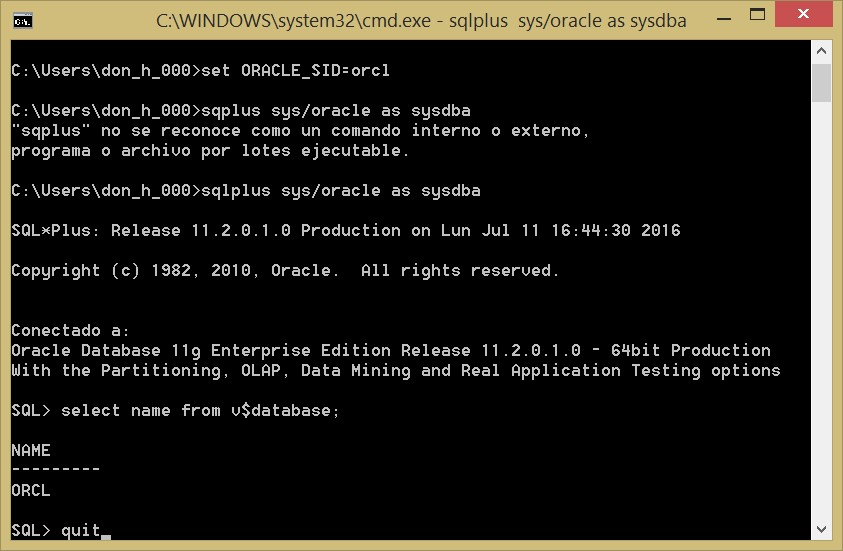
\includegraphics[width=7cm]{./Imagenes/b1}  
	\end{center}
	Una  vez  logueados  en  EM,  iremos  al  apartado Disponibilidad y  apuntaremos  a Planificar  Copia de Seguridad.
	\begin{center}
	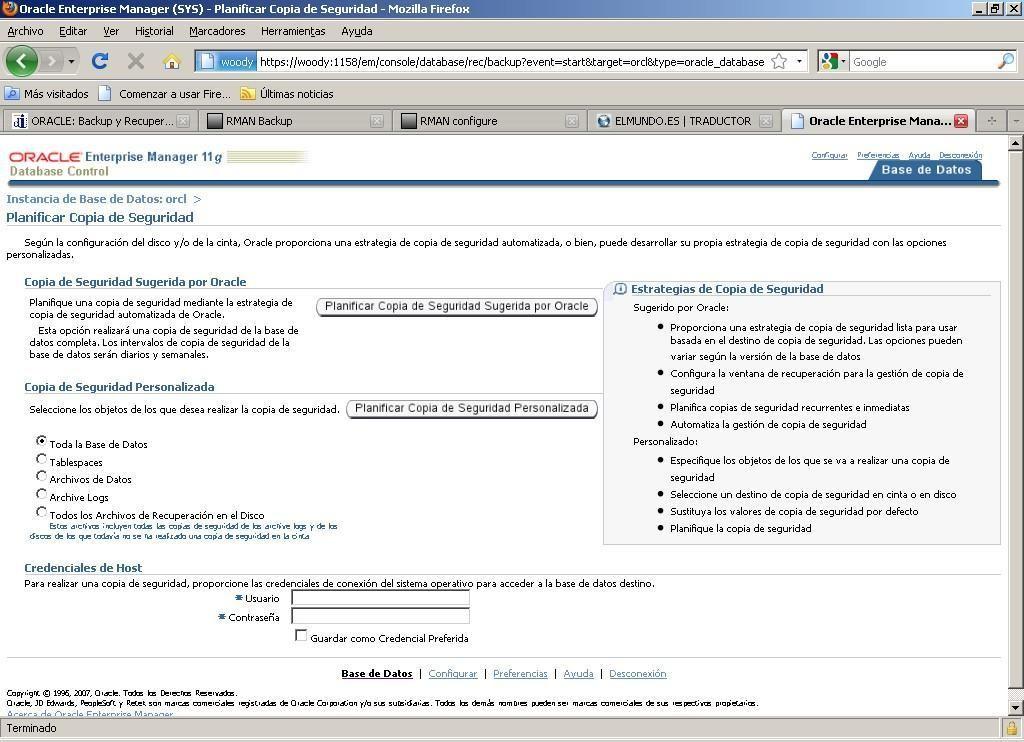
\includegraphics[width=7cm]{./Imagenes/b2}  
	\end{center}
	Figura 3. Como vemos nos da 2 opciones a elegir. En este documento analizaremos la opcion personalizada con toda la base de datos.
  	\\ Deberemos conectarnos con los credenciales de host para realizar esta tarea.
	\begin{center}
	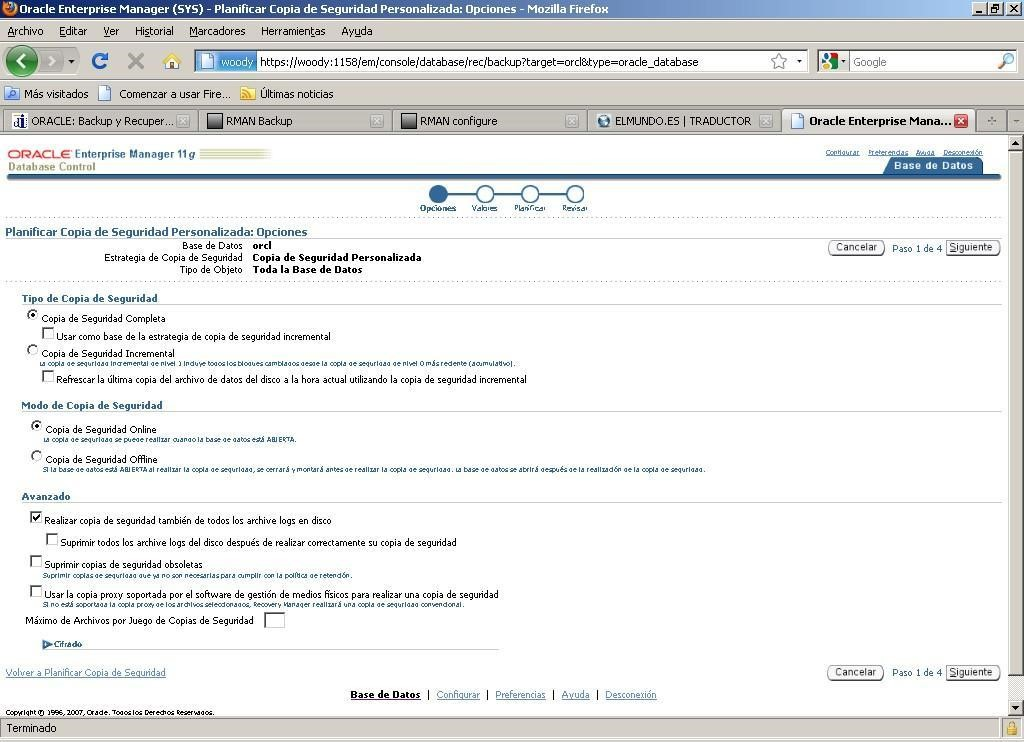
\includegraphics[width=7cm]{./Imagenes/b3}  
	\end{center}
	Figura 4. Como  es  la  primera  copia  que  realizamos  deberiamos  elegir  Copia  de  Seguridad Completa
	\\Para el modo de copia elegiremos si deseamos hacer la copia con la base de datos abierta o cerrada. En las opciones avanzadas tan solo agregaremos para que realice la copia tambien de los archive logs.
	\begin{center}
	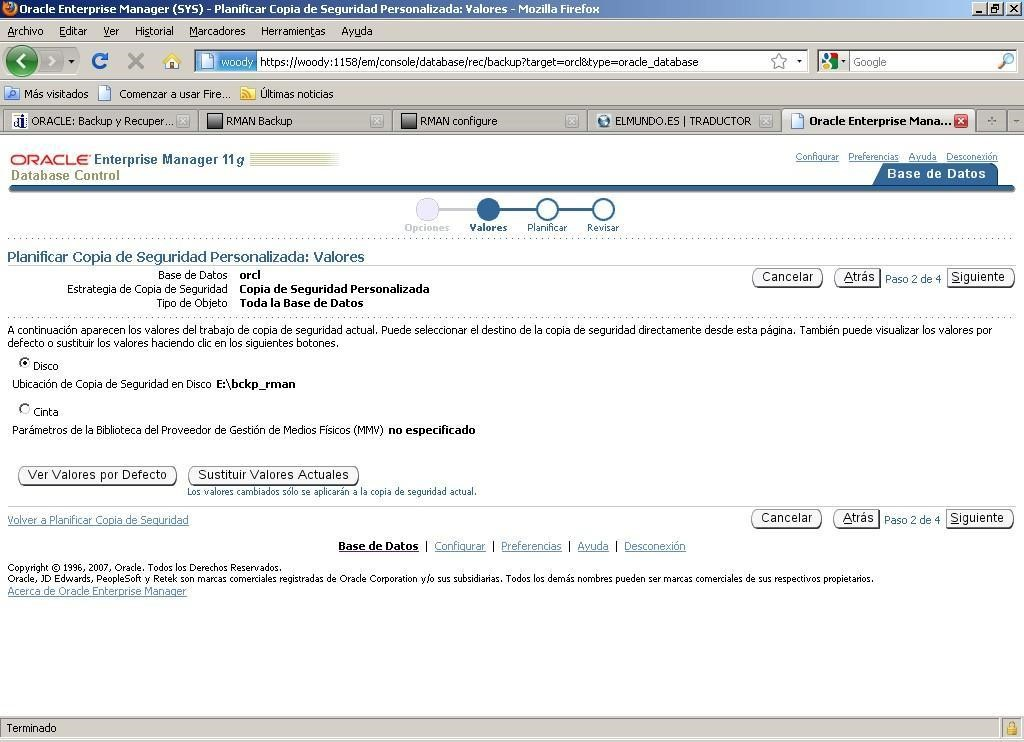
\includegraphics[width=7cm]{./Imagenes/b4}  
	\end{center}
	Figura 5. En este paso elegiremos el destino de la copia. Como no dispongo de dispositivo de cintas paso a continuar explicando la opcion Disco. (La ubicacion que ha tomado para la opcion Disco esta asignada desde RMAN).
	\begin{center}
	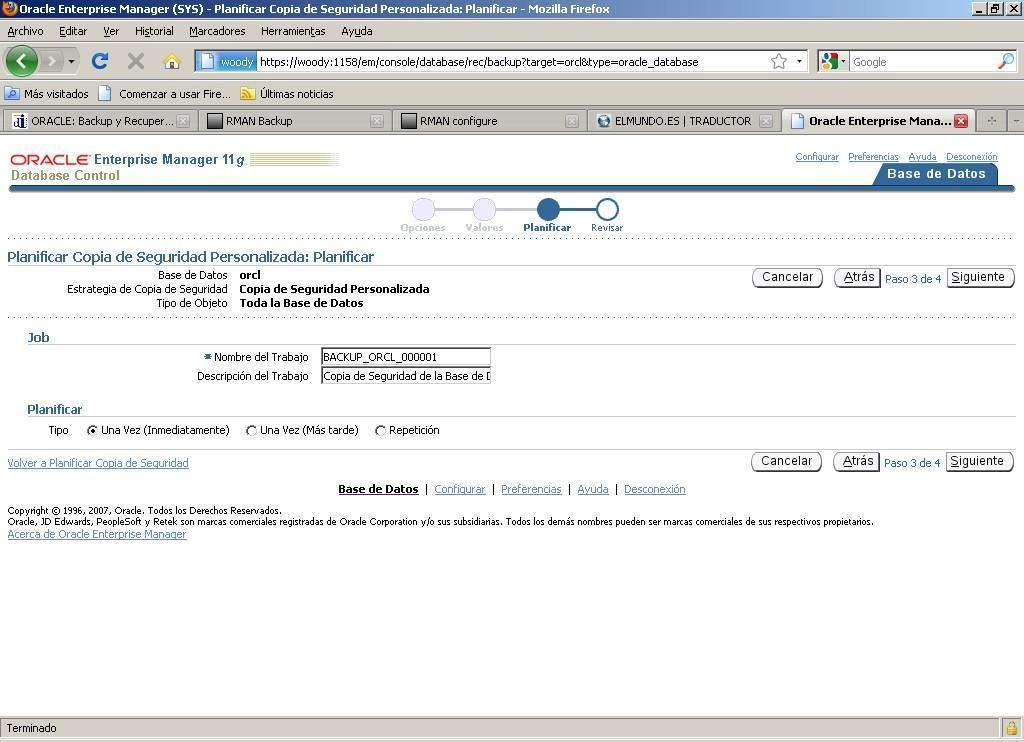
\includegraphics[width=7cm]{./Imagenes/b5}  
	\end{center}
	Figura 6. Introducimos nombre si lo deseamos y la descripcipn, y lo planificamos para que se realice una vez y de forma inmediata.
	\begin{center}
	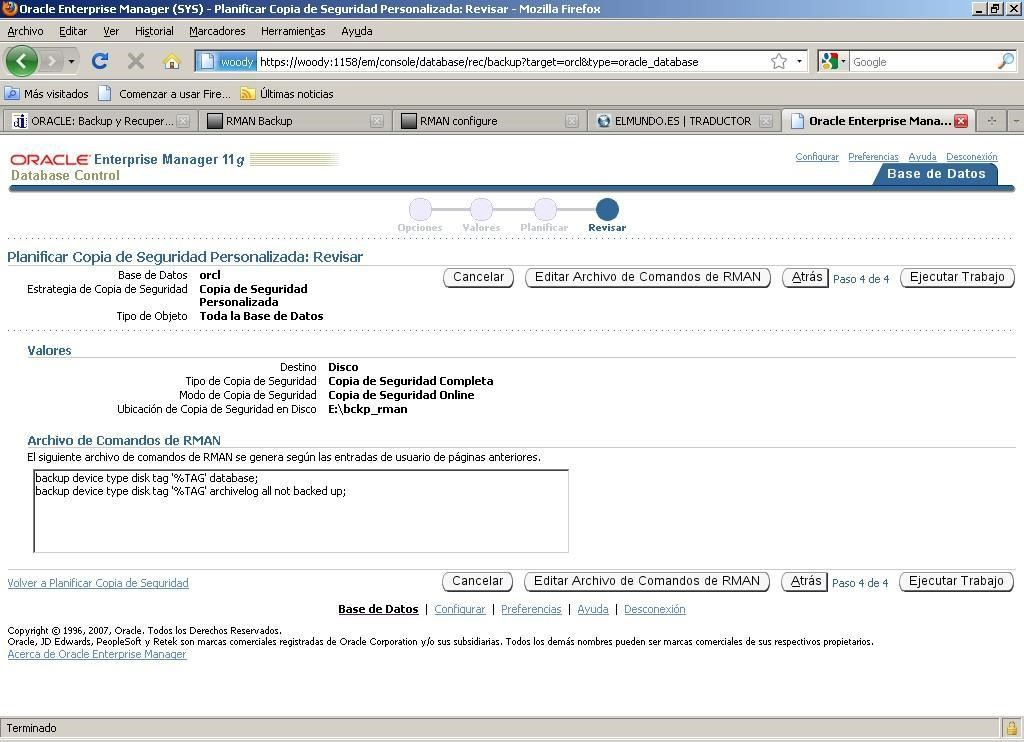
\includegraphics[width=7cm]{./Imagenes/b6}  
	\end{center}
	Figura 7. Revisamos que todo este correcto y ejecutamos el trabajo. Si todo ha ido bien deberia aparecer esto:
	\begin{center}
	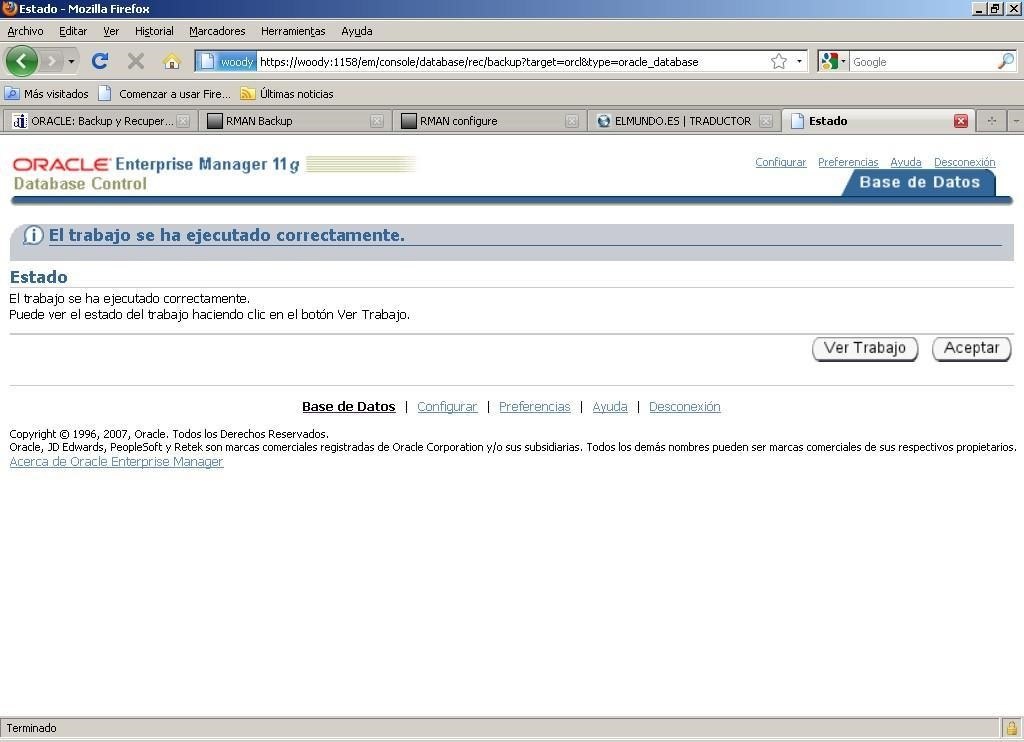
\includegraphics[width=7cm]{./Imagenes/b7}  
	\end{center}



\item RECUPERACION DESDE ENTERPRISE MANAGER
Para realizar una recuperacion desde EM, iremos a Disponibilidad y seleccionamos Realizar Recuperacin
\begin{center}
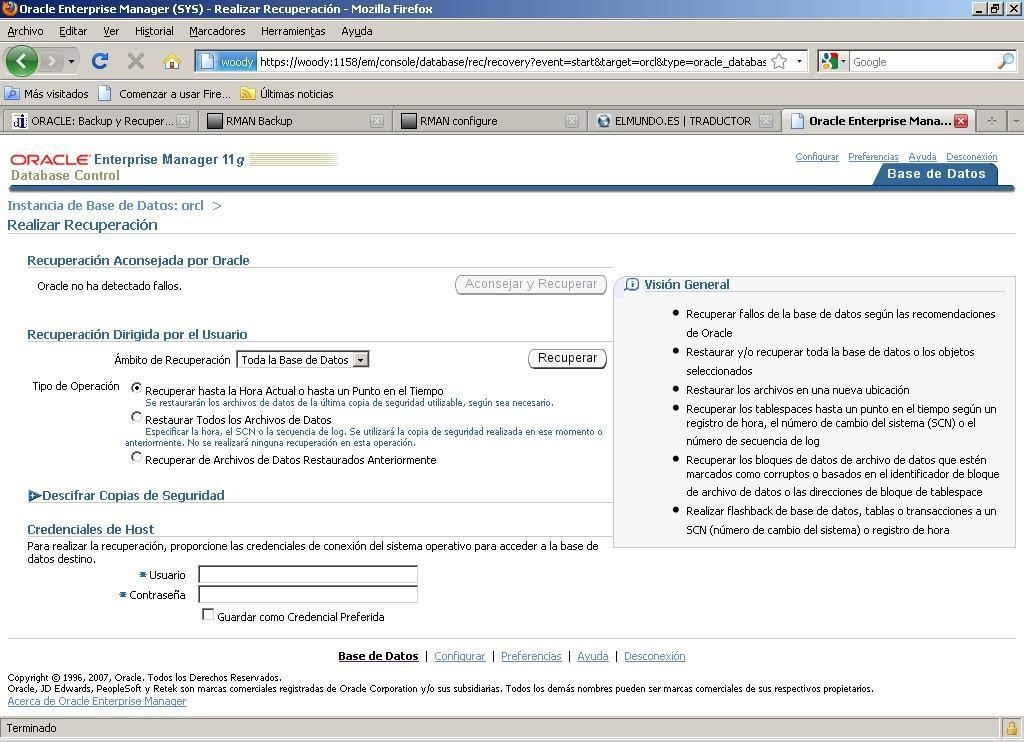
\includegraphics[width=7cm]{./Imagenes/r1} 
\end{center}
En ambitos de recuperacion podemos seleccionar toda o parte de la base de datos para recuperar
Para el ejemplo hemos borrado el datafile USERS01.DBF(OFFLINE) después de realizar el backup y ahora vamos a intentar recuperarlo. Para ello usaremos la copia que acabamos de realizar Iniciamos oracle en modo mount y arrancamos EM. Al no poder iniciar nos encontramos con esto una vez logueados
\begin{center}
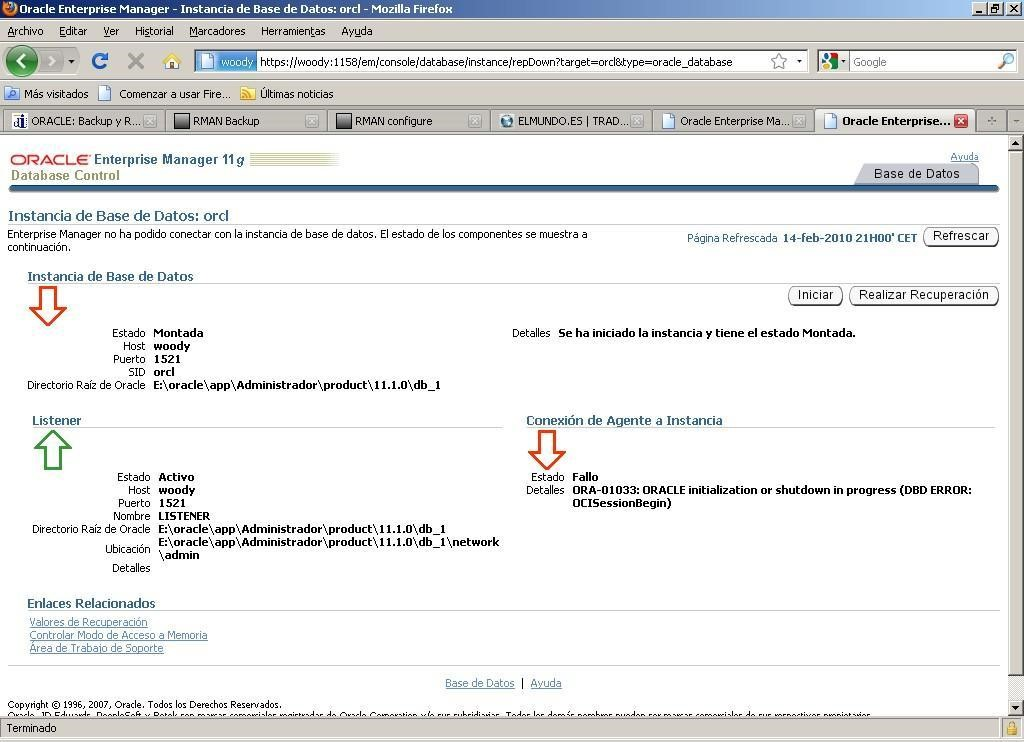
\includegraphics[width=7cm]{./Imagenes/r2} 
\end{center}
Selecionamos en Realizar Recuperacion y Introducimos las credenciales de host. Continuar Nos conectamos como sysdba.
\begin{center}
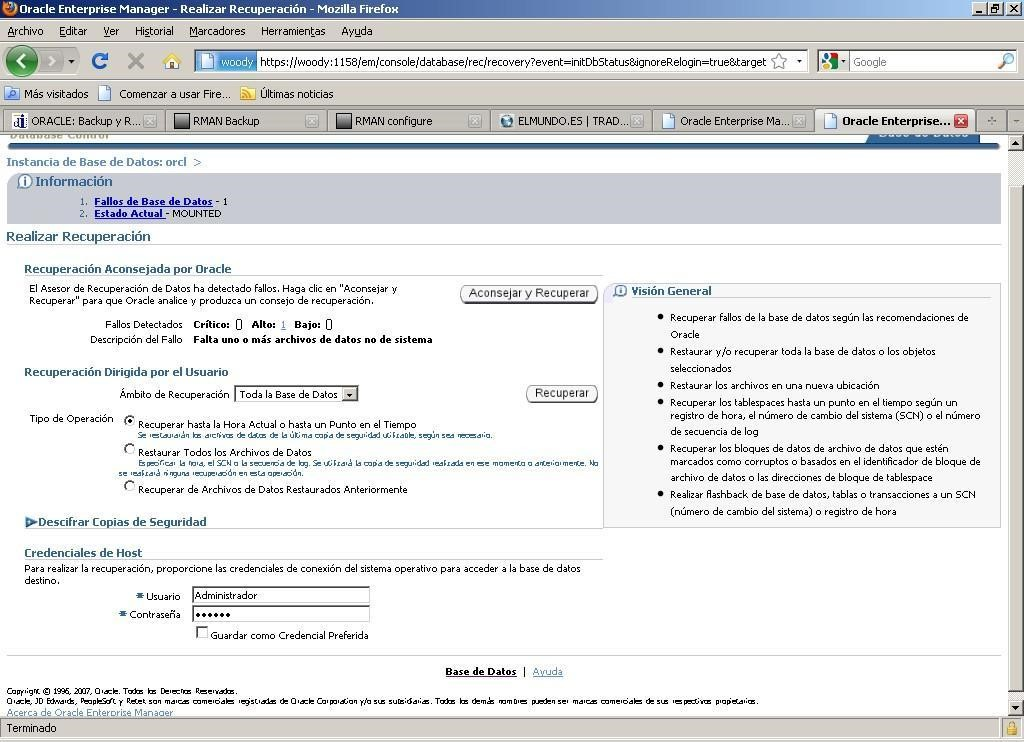
\includegraphics[width=7cm]{./Imagenes/r3} 
\end{center}
En el ambito de recuperacion elegimos Archivos de Datos y en el tipo de operacion restaurar hasta hora actual. Seleccionamos en recuperar.
\begin{center}
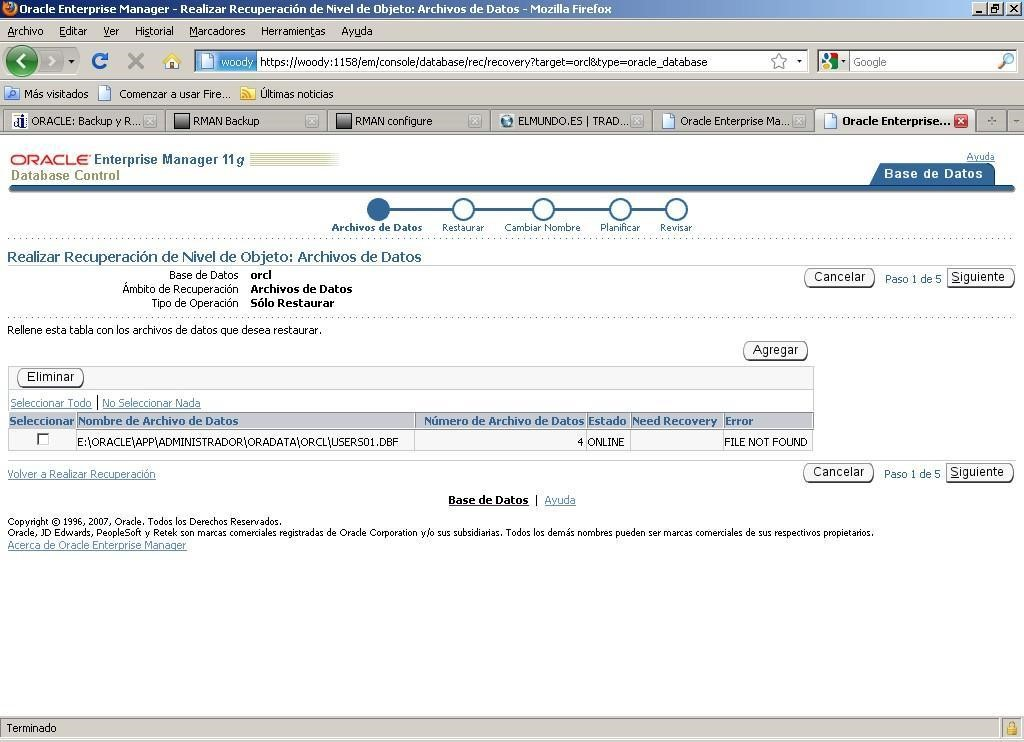
\includegraphics[width=7cm]{./Imagenes/r4} 
\end{center} 




\end{enumerate} 

         Vemos como EM localiza la ruta en conflicto y te la presenta para sleccionarla. Siguiente.\\ \\
          \begin{center}
          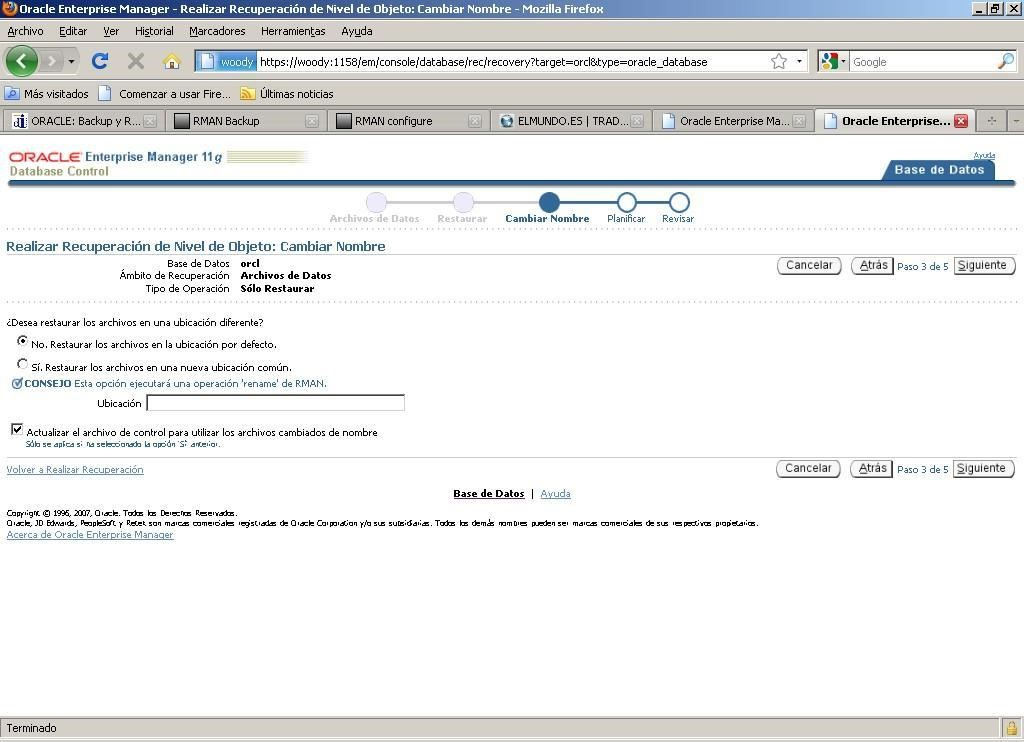
\includegraphics[width=7cm]{./Imagenes/recu_5.jpg}
          \end{center}
          \normalsize Tambi\'en podemos definir el destino de la restauraci\'on. Para el ejemplo  nos interesa que se ubiquen en el mismo directorio. \\ 

         \begin{center}
          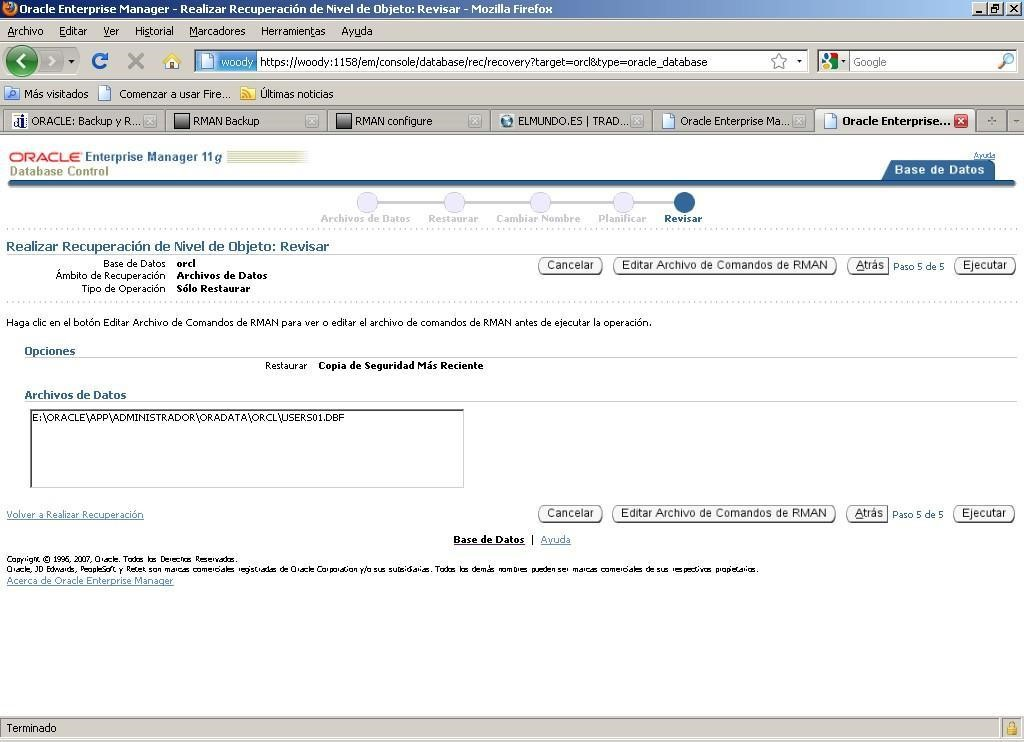
\includegraphics[width=7cm]{./Imagenes/recu_6.jpg}
           \end{center}

           \normalsize Podemos revisar los par\'ametros RMAN para ver y comprender las acciones realizadas por debajo de EM. Una vez este revisado procederemos a ejecutar. 
 Esto lo que har\'a ser\'a tomar del backup el fichero y llevarlo al destino aplicando los cambios hasta el momento de la p\'erdida permitiendo as\'i el inicio normal de la BD con tablespace online. 
Una vez finalizado podemos pinchar en Abrir Base de Datos y esta se reiniciar\'a y se abrira automaticamente despues de ver insertado nuestros credenciales.\\ 
\begin{center}
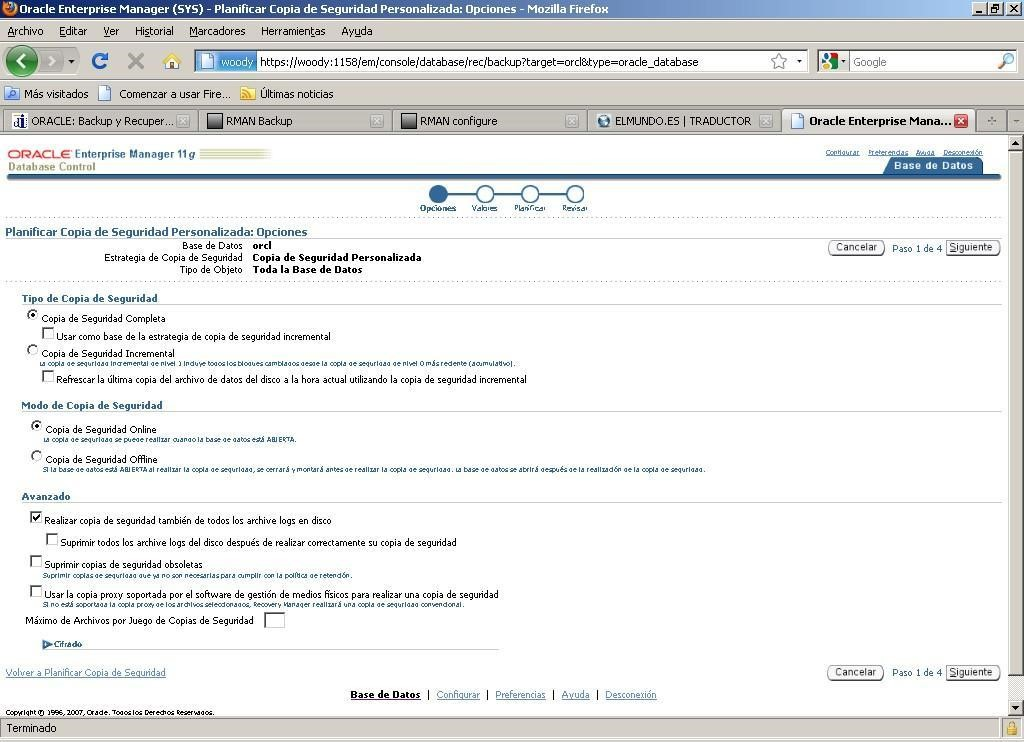
\includegraphics[width=7cm]{./Imagenes/eje1.jpg}
 \end{center}
 En este paso elegiremos el destino de la copia, como no disponemos del dispositivo de cintas , se pasa a continuar explicando la opci\'on Disco. La ubicacion que ha tomado para la opci\'on 
Disco esta asignada desde RMAN.
\begin{center}
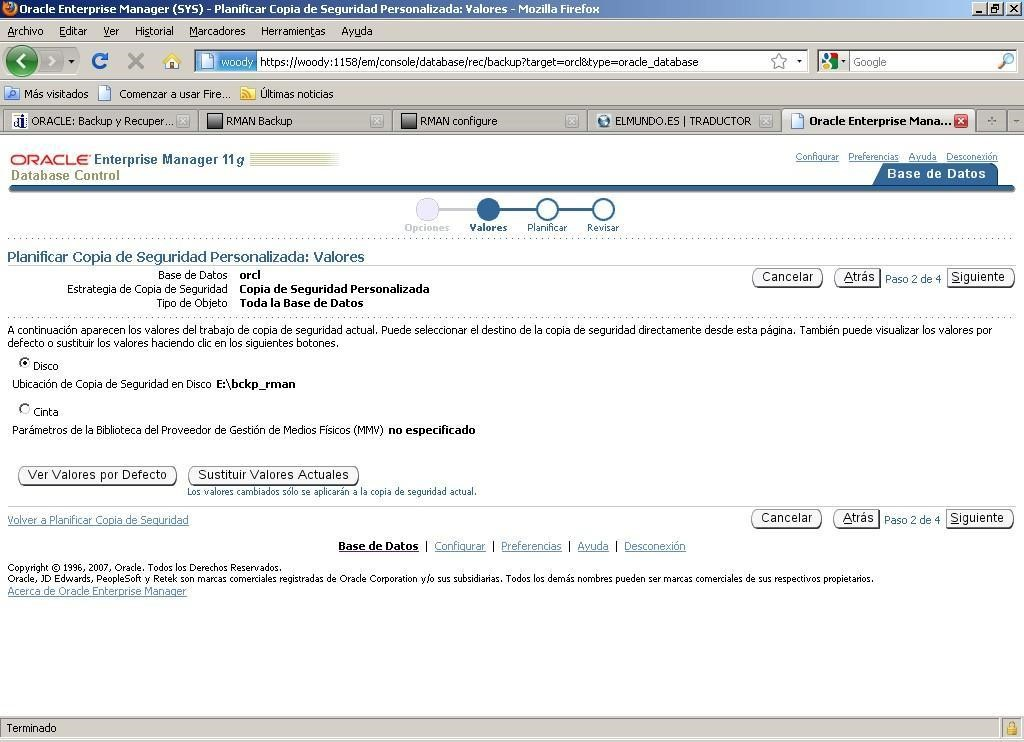
\includegraphics[width=7cm]{./Imagenes/eje2.jpg}
\end{center}

 Introducimos nombre si lo deseamos y la descripci\'on, y lo planificamos para que se realice una vez y de forma inmediata.
\begin{center}
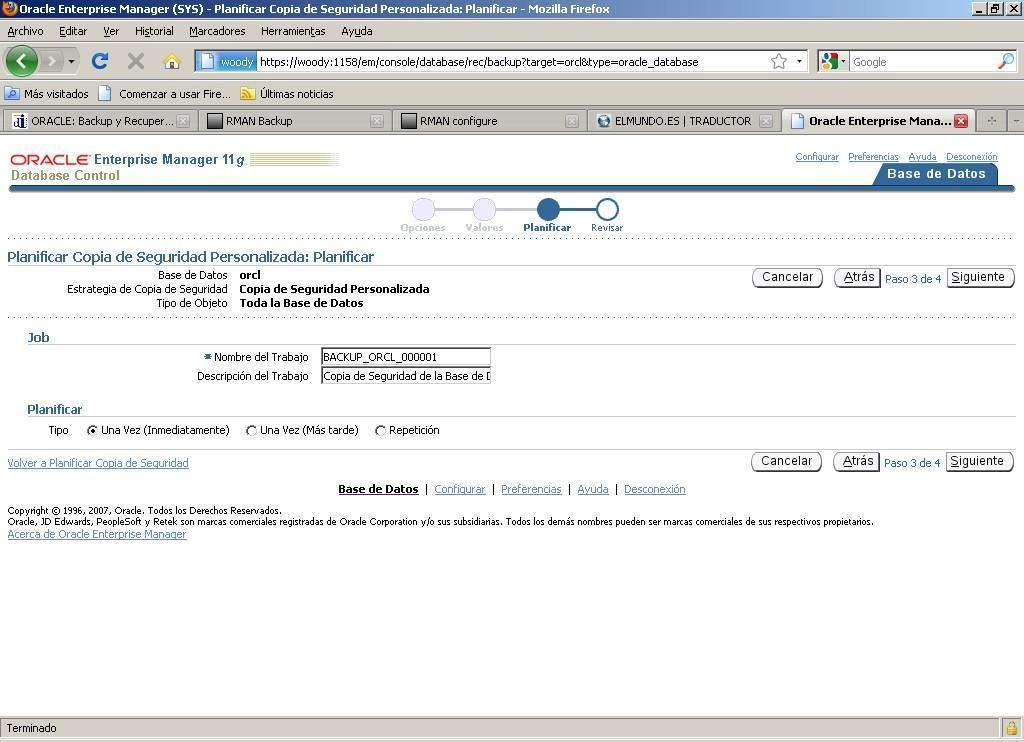
\includegraphics[width=7cm]{./Imagenes/eje3.jpg}
\end{center}
Revisamos que todo este correcto y ejecutamos el trabajo. Si todo ha sido correcto deberia aparecer esto.\\
\begin{center}
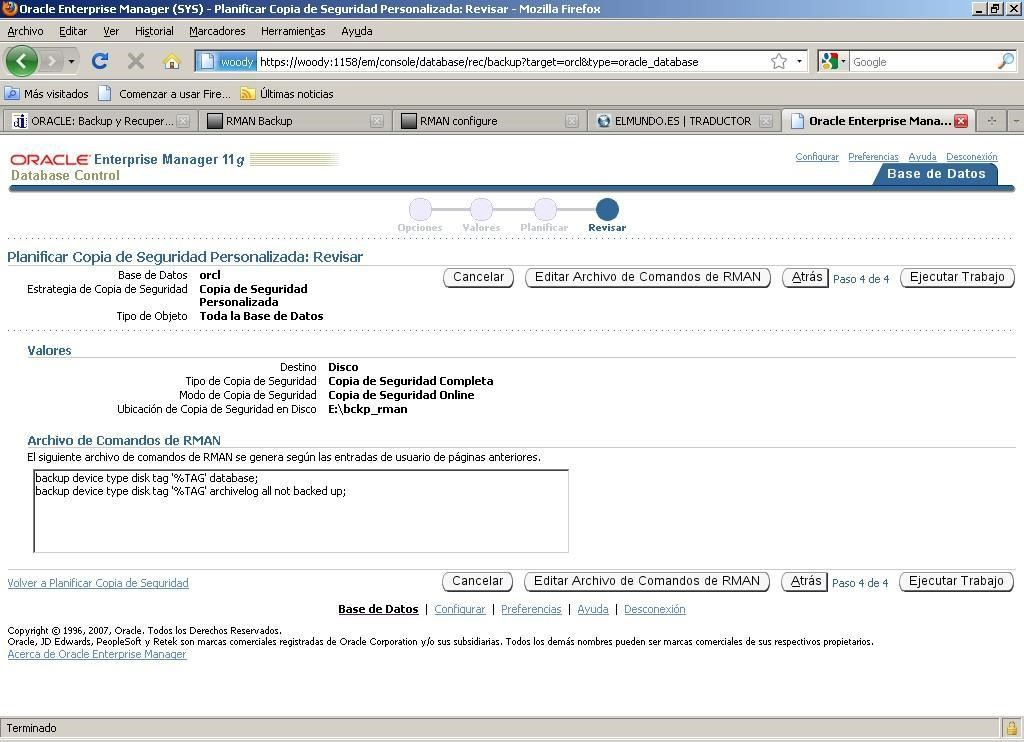
\includegraphics[width=7cm]{./Imagenes/eje4.jpg}
\end{center}
Recuperacion desde Enterprise Manager
Para realizar una recuperaci\'on desde EM , iremos a Disponibilidad y seleccionamos "Realizar Recuperaci\'on".\\
\begin{center}
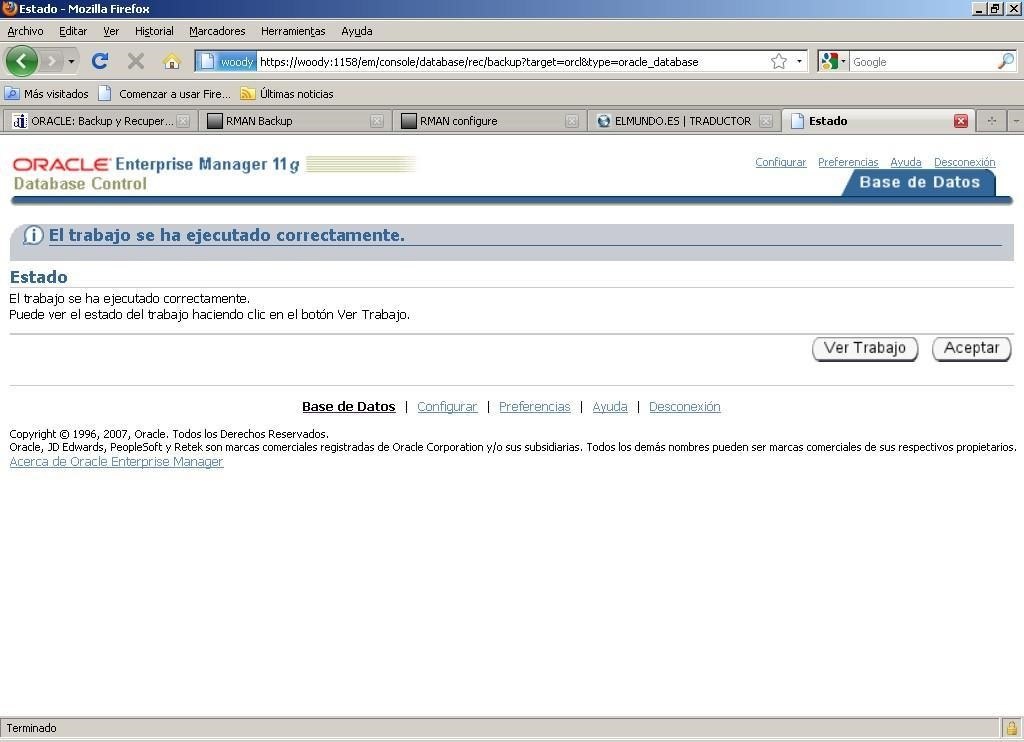
\includegraphics[width=7cm]{./Imagenes/eje5.jpg}
\end{center}
Iniciamos oracle en modo mount y arracamos EM.\\
\begin{center}
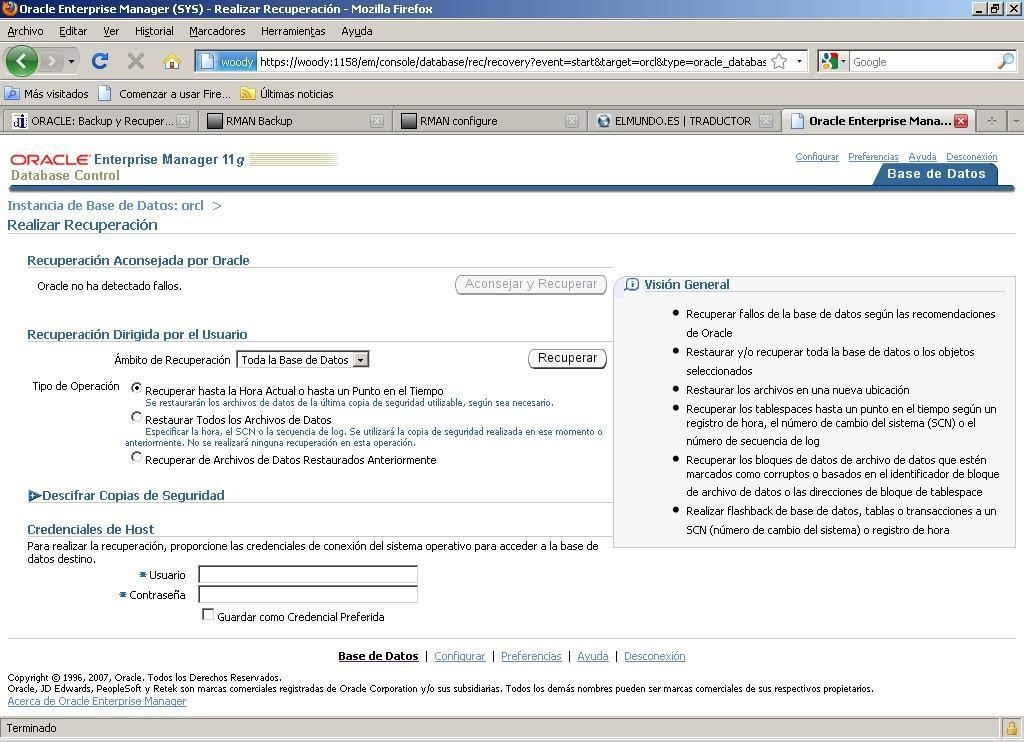
\includegraphics[width=7cm]{./Imagenes/eje6.jpg}
\end{center}

Pinchamos en Realizar Recuperacion. Seguidamente introducimos las credenciales de host. Continuar. Nos conectamos como sysdba.
\begin{center}
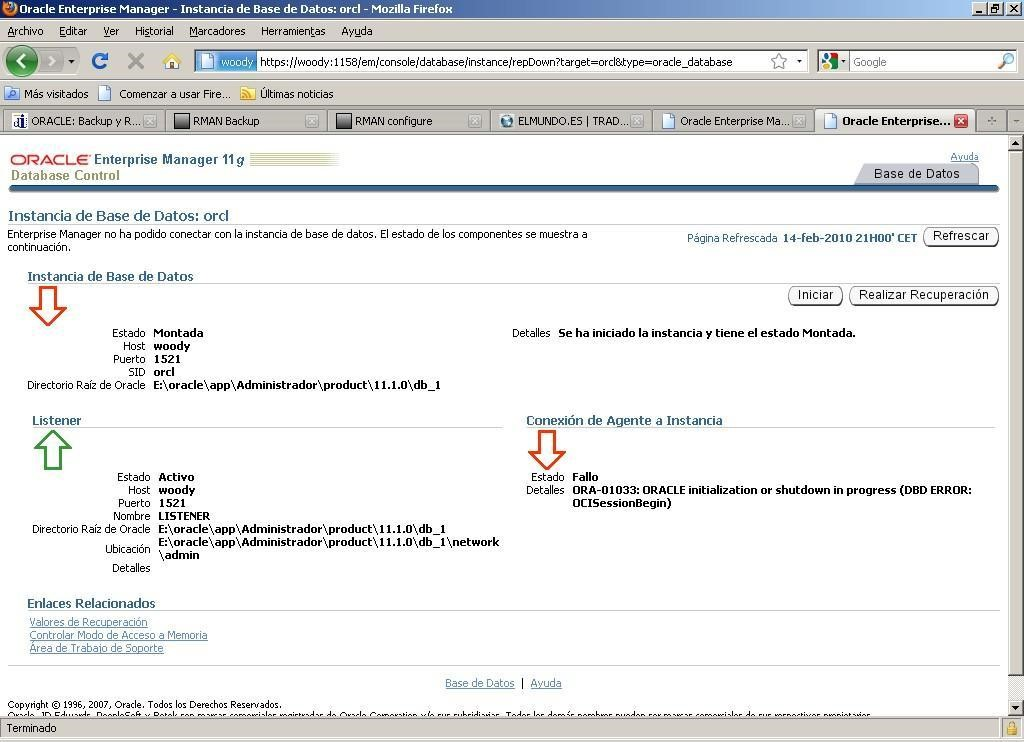
\includegraphics[width=7cm]{./Imagenes/eje7.jpg}
\end{center}
En el \'ambito de recuperacion elegimos Archivos de Datos y en el tipo de operaci\'on restaurar hasta hora actual. Pinchamos en recuperar
\begin{center}
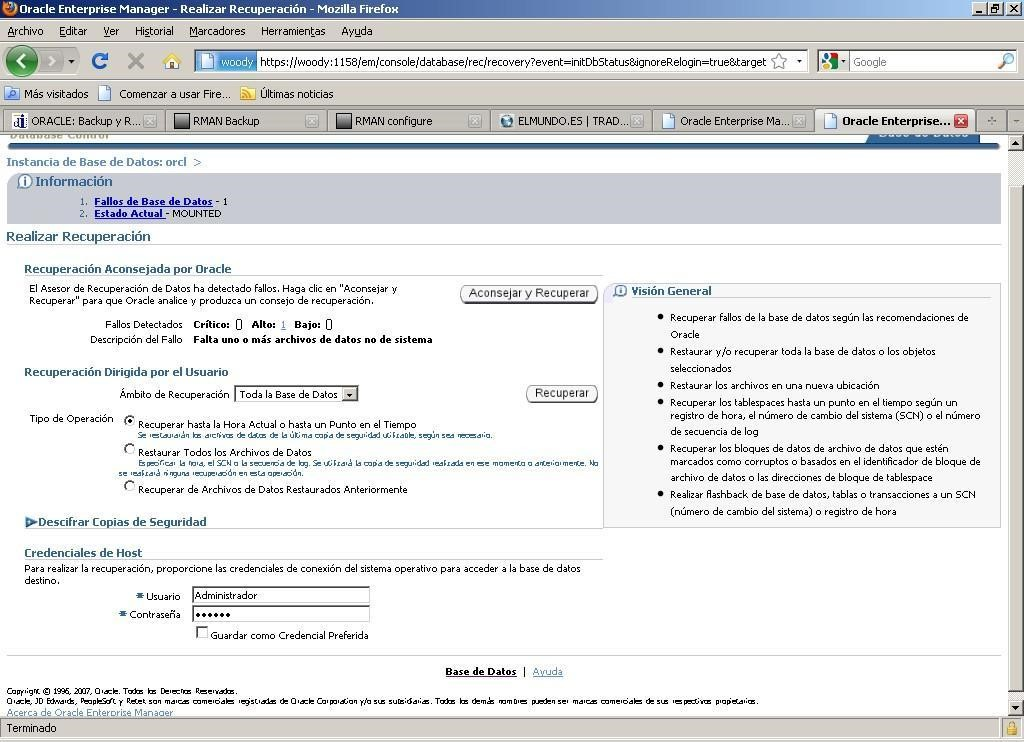
\includegraphics[width=7cm]{./Imagenes/eje8.jpg}
\end{center}
      
\section{Referencias}
   \begin{enumerate}[a)]
        \item Biliograf\'ia
\begin{itemize}  
\normalsize \item `` An\'alisis y Configuraci\'on de un Plan de Respaldo de Base de Datos Oracle 11g Usando Metodolog\'ia
(Rman y Datapump) para la Administraci\'on de Backup en DM2 Consulting ''
AVILA BERNARDO, HILDA MERY, 2015
\item  Copias de seguridad y restauraci\'on. Por Ra\'ul Lobo Medinilla, IES Gonzalo Nazareno p\'ag. No02
\item Oracle Database 11g en Windows: Desarrollo e Implementaci\'on.pdf

\end{itemize}
\normalsize	\item Art\'iculos
\begin{itemize}  
 \item \normalsize https://searchdatacenter.techtarget.com
\normalsize es/cronica/Copia-de-seguridad-completa-incremental-o-diferencial-como-
\normalsize elegir-el-tipo-adecuado
\normalsize \item http://www.ajpdsoft.com/modules.php?
\normalsize name=News\&file=article\&sid=560
\normalsize \item https://www.infor.uva.es/
\end{itemize}
 \end{enumerate}




\section{Conclusiones}
\begin{itemize}  
\item Se pueden realizar backups con la base de datos conectada o desconectada ademas de por
modo consola o grafica con el Enterprise Manager
\item La planeaci\'on de una buena estrategia de backup y de restauraci\'on es imprescindible para
agilizar la restauraci\'on de informaci\'on
\item Una estrategia de backup va a depender de los datos a respaldar
\end{itemize}

\end{document}